\documentclass[12pt]{article}

%%%% packages and definitions (optional)
\usepackage{graphicx} % allows inclusion of graphics
\usepackage{graphics}
\usepackage{placeins}
\usepackage{booktabs} % nice rules (thick lines) for tables
\usepackage{microtype} % improves typography for PDF
\usepackage{xspace}
\usepackage[hidelinks]{hyperref}
\usepackage{xspace}
\usepackage{hhline}
\usepackage{multirow}

\usepackage{pgfgantt}
\usepackage{rotating}
\usepackage[graphicx]{realboxes}
\usepackage{lscape}
\usepackage[margin=0.5in,landscape]{geometry}
\usepackage{wrapfig}
\usepackage{lipsum}

\def\pgfcalendarweekdayletter#1{%  
 \ifcase#1M\or Tu\or W\or Tr\or F\or Sa\or Su\fi%  
}  
\usepackage{amsmath}

\usepackage{tabularx}
\newcolumntype{b}{>{\hsize=1.0\hsize}X}
\newcolumntype{s}{>{\hsize=.5\hsize}X}
\newcolumntype{m}{>{\hsize=.75\hsize}X}

\newcommand{\SN}{S$_N$}
\renewcommand{\vec}[1]{\bm{#1}} %vector is bold italic
\newcommand{\vd}{\bm{\cdot}} % slightly bold vector dot
\newcommand{\grad}{\vec{\nabla}} % gradient
\newcommand{\ud}{\mathop{}\!\mathrm{d}} % upright derivative symbol
\newcommand{\Cyclus}{\textsc{Cyclus}\xspace}%
\graphicspath{ {images/} }
\usepackage[affil-it]{authblk}
\usepackage[numbers]{natbib}
\usepackage{notoccite}
\usepackage{tikz}
\usetikzlibrary{positioning, arrows, decorations, shapes }
\usepackage{cleveref}

\usepackage{datatool}
\usepackage[acronym,toc]{glossaries}
%\newacronym{<++>}{<++>}{<++>}
\newacronym[longplural={metric tons of heavy metal}]{MTHM}{MTHM}{metric ton of heavy metal}
\newacronym{ABM}{ABM}{agent-based modeling}
\newacronym{ACDIS}{ACDIS}{Program in Arms Control \& Domestic and International Security}
\newacronym{ADS}{ADS}{Accelerator-Driven Systems}
\newacronym{AHTR}{AHTR}{Advanced High Temperature Reactor}
\newacronym{ANDRA}{ANDRA}{Agence Nationale pour la gestion des D\'echets RAdioactifs, the French National Agency for Radioactive Waste Management}
\newacronym{ANL}{ANL}{Argonne National Laboratory}
\newacronym{ANS}{ANS}{American Nuclear Society}
\newacronym{API}{API}{application programming interface}
\newacronym{ARE}{ARE}{Aircraft Reactor Experiment}
\newacronym{ARFC}{ARFC}{Advanced Reactors and Fuel Cycles}
\newacronym{ASME}{ASME}{American Society of Mechanical Engineers}
\newacronym{ATWS}{ATWS}{Anticipated Transient Without Scram}
\newacronym{BDBE}{BDBE}{Beyond Design Basis Event}
\newacronym{BIDS}{BIDS}{Berkeley Institute for Data Science}
\newacronym{BWR}{BWR}{Boiling Water Reactor}
\newacronym{CAFCA}{CAFCA}{ Code for Advanced Fuel Cycles Assessment }
\newacronym{CDTN}{CDTN}{Centro de Desenvolvimento da Tecnologia Nuclear}
\newacronym{CEA}{CEA}{Commissariat \`a l'\'Energie Atomique et aux \'Energies Alternatives}
\newacronym{CI}{CI}{continuous integration}
\newacronym{CNEN}{CNEN}{Comiss\~{a}o Nacional de Energia Nuclear}
\newacronym{CNERG}{CNERG}{Computational Nuclear Engineering Research Group}
\newacronym{COSI}{COSI}{Commelini-Sicard}
\newacronym{COTS}{COTS}{commercial, off-the-shelf}
\newacronym{CSNF}{CSNF}{commercial spent nuclear fuel}
\newacronym{CTAH}{CTAHs}{Coiled Tube Air Heaters}
\newacronym{CUBIT}{CUBIT}{CUBIT Geometry and Mesh Generation Toolkit}
\newacronym{CURIE}{CURIE}{Centralized Used Fuel Resource for Information Exchange}
\newacronym{DAG}{DAG}{directed acyclic graph}
\newacronym{DANESS}{DANESS}{Dynamic Analysis of Nuclear Energy System Strategies}
\newacronym{DBE}{DBE}{Design Basis Event}
\newacronym{DESAE}{DESAE}{Dynamic Analysis of Nuclear Energy Systems Strategies}
\newacronym{DHS}{DHS}{Department of Homeland Security}
\newacronym{DOE}{DOE}{Department of Energy}
\newacronym{DRACS}{DRACS}{Direct Reactor Auxiliary Cooling System}
\newacronym{DRE}{DRE}{dynamic resource exchange}
\newacronym{DSNF}{DSNF}{DOE spent nuclear fuel}
\newacronym{DYMOND}{DYMOND}{Dynamic Model of Nuclear Development }
\newacronym{EBS}{EBS}{Engineered Barrier System}
\newacronym{EDF}{EDF}{Électricité de France}
\newacronym{EDZ}{EDZ}{Excavation Disturbed Zone}
\newacronym{EIA}{EIA}{U.S. Energy Information Administration}
\newacronym{EPA}{EPA}{Environmental Protection Agency}
\newacronym{EPR}{EPR}{European Pressurized Reactor}
\newacronym{EP}{EP}{Engineering Physics}
\newacronym{EU}{EU}{European Union}
\newacronym{FCO}{FCO}{Fuel Cycle Options}
\newacronym{FCT}{FCT}{Fuel Cycle Technology}
\newacronym{FEHM}{FEHM}{Finite Element Heat and Mass Transfer}
\newacronym{FEPs}{FEPs}{Features, Events, and Processes}
\newacronym{FHR}{FHR}{Fluoride-Salt-Cooled High-Temperature Reactor}
\newacronym{FLiBe}{FLiBe}{Fluoride-Lithium-Beryllium}
\newacronym{FP}{FP}{Fission Products}
\newacronym{GDSE}{GDSE}{Generic Disposal System Environment}
\newacronym{GDSM}{GDSM}{Generic Disposal System Model}
\newacronym{GENIUSv1}{GENIUSv1}{Global Evaluation of Nuclear Infrastructure Utilization Scenarios, Version 1}
\newacronym{GENIUSv2}{GENIUSv2}{Global Evaluation of Nuclear Infrastructure Utilization Scenarios, Version 2}
\newacronym{GENIUS}{GENIUS}{Global Evaluation of Nuclear Infrastructure Utilization Scenarios}
\newacronym{GPAM}{GPAM}{Generic Performance Assessment Model}
\newacronym{GRSAC}{GRSAC}{Graphite Reactor Severe Accident Code}
\newacronym{GUI}{GUI}{graphical user interface}
\newacronym{HLW}{HLW}{high level waste}
\newacronym{HPC}{HPC}{high-performance computing}
\newacronym{HTC}{HTC}{high-throughput computing}
\newacronym{HTGR}{HTGR}{High Temperature Gas-Cooled Reactor}
\newacronym{IAEA}{IAEA}{International Atomic Energy Agency}
\newacronym{IEMA}{IEMA}{Illinois Emergency Mangament Agency}
\newacronym{IHLRWM}{IHLRWM}{International High Level Radioactive Waste Management}
\newacronym{INL}{INL}{Idaho National Laboratory}
\newacronym{IPRR1}{IRP-R1}{Instituto de Pesquisas Radioativas Reator 1}
\newacronym{IRP}{IRP}{Integrated Research Project}
\newacronym{ISFSI}{ISFSI}{Independent Spent Fuel Storage Installation}
\newacronym{ISRG}{ISRG}{Independent Student Research Group}
\newacronym{JFNK}{JFNK}{Jacobian-Free Newton Krylov}
\newacronym{LANL}{LANL}{Los Alamos National Laboratory}
\newacronym{LBNL}{LBNL}{Lawrence Berkeley National Laboratory}
\newacronym{LCOE}{LCOE}{levelized cost of electricity}
\newacronym{LDRD}{LDRD}{laboratory directed research and development}
\newacronym{LFR}{LFR}{Lead-Cooled Fast Reactor}
\newacronym{LLNL}{LLNL}{Lawrence Livermore National Laboratory}
\newacronym{LMFBR}{LMFBR}{Liquid Metal Fast Breeder Reactor}
\newacronym{LOFC}{LOFC}{Loss of Forced Cooling}
\newacronym{LOHS}{LOHS}{Loss of Heat Sink}
\newacronym{LOLA}{LOLA}{Loss of Large Area}
\newacronym{LP}{LP}{linear program}
\newacronym{LWR}{LWR}{Light Water Reactor}
\newacronym{MAGNOX}{MAGNOX}{Magnesium Alloy Graphie Moderated Gas Cooled Uranium Oxide Reactor}
\newacronym{MA}{MA}{minor actinide}
\newacronym{MCNP}{MCNP}{Monte Carlo N-Particle code}
\newacronym{MILP}{MILP}{mixed-integer linear program}
\newacronym{MIT}{MIT}{the Massachusetts Institute of Technology}
\newacronym{MOAB}{MOAB}{Mesh-Oriented datABase}
\newacronym{MOOSE}{MOOSE}{Multiphysics Object-Oriented Simulation Environment}
\newacronym{MOX}{MOX}{Mixed Oxide Fuel}
\newacronym{MSBR}{MSBR}{Molten Salt Breeder Reactor}
\newacronym{MSRE}{MSRE}{Molten Salt Reactor Experiment}
\newacronym{MSR}{MSR}{Molten Salt Reactor}
\newacronym{NAGRA}{NAGRA}{National Cooperative for the Disposal of Radioactive Waste}
\newacronym{NEAMS}{NEAMS}{Nuclear Engineering Advanced Modeling and Simulation}
\newacronym{NEUP}{NEUP}{Nuclear Energy University Programs}
\newacronym{NFCSim}{NFCSim}{Nuclear Fuel Cycle Simulator}
\newacronym{NGNP}{NGNP}{Next Generation Nuclear Plant}
\newacronym{NMWPC}{NMWPC}{Nuclear MW Per Capita}
\newacronym{NNSA}{NNSA}{National Nuclear Security Administration}
\newacronym{NPRE}{NPRE}{Department of Nuclear, Plasma, and Radiological Engineering}
\newacronym{NQA1}{NQA-1}{Nuclear Quality Assurance - 1}
\newacronym{NRC}{NRC}{Nuclear Regulatory Commission}
\newacronym{NSF}{NSF}{National Science Foundation}
\newacronym{NSSC}{NSSC}{Nuclear Science and Security Consortium}
\newacronym{NUWASTE}{NUWASTE}{Nuclear Waste Assessment System for Technical Evaluation}
\newacronym{NWF}{NWF}{Nuclear Waste Fund}
\newacronym{NWTRB}{NWTRB}{Nuclear Waste Technical Review Board}
\newacronym{OCRWM}{OCRWM}{Office of Civilian Radioactive Waste Management}
\newacronym{ORION}{ORION}{ORION}
\newacronym{ORNL}{ORNL}{Oak Ridge National Laboratory}
\newacronym{PARCS}{PARCS}{Purdue Advanced Reactor Core Simulator}
\newacronym{PBAHTR}{PB-AHTR}{Pebble Bed Advanced High Temperature Reactor}
\newacronym{PBFHR}{PB-FHR}{Pebble-Bed Fluoride-Salt-Cooled High-Temperature Reactor}
\newacronym{PEI}{PEI}{Peak Environmental Impact}
\newacronym{PH}{PRONGHORN}{PRONGHORN}
\newacronym{PRA}{PRA}{probabilistic risk assessment}
\newacronym{PRIS}{PRIS}{Power Reactor Information System}
\newacronym{PRKE}{PRKE}{Point Reactor Kinetics Equations}
\newacronym{PSPG}{PSPG}{Pressure-Stabilizing/Petrov-Galerkin}
\newacronym{PWAR}{PWAR}{Pratt and Whitney Aircraft Reactor}
\newacronym{PWR}{PWR}{Pressurized Water Reactor}
\newacronym{PyNE}{PyNE}{Python toolkit for Nuclear Engineering}
\newacronym{PyRK}{PyRK}{Python for Reactor Kinetics}
\newacronym{QA}{QA}{quality assurance}
\newacronym{RDD}{RD\&D}{Research Development and Demonstration}
\newacronym{RD}{R\&D}{Research and Development}
\newacronym{RELAP}{RELAP}{Reactor Excursion and Leak Analysis Program}
\newacronym{RIA}{RIA}{Reactivity Insertion Accident}
\newacronym{RIF}{RIF}{Region-Institution-Facility}
\newacronym{SFR}{SFR}{Sodium-Cooled Fast Reactor}
\newacronym{SINDAG}{SINDA{\textbackslash}G}{Systems Improved Numerical Differencing Analyzer $\backslash$ Gaski}
\newacronym{SKB}{SKB}{Svensk K\"{a}rnbr\"{a}nslehantering AB}
\newacronym{SNF}{SNF}{spent nuclear fuel}
\newacronym{SNL}{SNL}{Sandia National Laboratory}
\newacronym{STC}{STC}{specific temperature change}
\newacronym{SUPG}{SUPG}{Streamline-Upwind/Petrov-Galerkin}
\newacronym{SWF}{SWF}{Separations and Waste Forms}
\newacronym{SWU}{SWU}{Separative Work Unit}
\newacronym{TRIGA}{TRIGA}{Training Research Isotope General Atomic}
\newacronym{TRISO}{TRISO}{Tristructural Isotropic}
\newacronym{TSM}{TSM}{Total System Model}
\newacronym{TSPA}{TSPA}{Total System Performance Assessment for the Yucca Mountain License Application}
\newacronym{ThOX}{ThOX}{thorium oxide}
\newacronym{UFD}{UFD}{Used Fuel Disposition}
\newacronym{UML}{UML}{Unified Modeling Language}
\newacronym{UNF}{UNF}{Used Nuclear Fuel}
\newacronym{UOX}{UOX}{Uranium Oxide Fuel}
\newacronym{UQ}{UQ}{uncertainty quantification}
\newacronym{US}{US}{United States}
\newacronym{UW}{UW}{University of Wisconsin}
\newacronym{VISION}{VISION}{the Verifiable Fuel Cycle Simulation Model}
\newacronym{VVER}{VVER}{Voda-Vodyanoi Energetichesky Reaktor (Russian Pressurized Water Reactor)}
\newacronym{VV}{V\&V}{verification and validation}
\newacronym{WIPP}{WIPP}{Waste Isolation Pilot Plant}
\newacronym{YMR}{YMR}{Yucca Mountain Repository Site}

	
\makeglossaries

\title{Modeling Methods for Initiating Events in Nuclear Spent Fuel Repositories}
\author{Jin Whan Bae}
\affil{Dept. of Nuclear, Plasma, and Radiological Engineering, University of Illinois at Urbana-Champaign
		  Urbana, IL}
\date{}                     %% if you don't need date to appear
\setcounter{Maxaffil}{0}
\renewcommand\Affilfont{\itshape\small}
%%%%%%%%%%%%%%actual words%%%%%%%%%%%%%%%%%%%%%%%%%%%%%%%%%%%%%%%%%%%%%%%%%%%%5


\begin{document}
\maketitle

\section{Abstract}
\gls{UNF} repositories, given the high decay heat and radioactivity
of \glspl{UNF}, requires careful engineering. The current plan is
to design a repository that would contain the material for one million years.
Considering various events (failures) can occur in that time range,
the \gls{UNF} repository proposes an interesting subject for
\gls{PRA}. In this report, the model repository design is after the 
\gls{YMR}, which is a mined repository in volcanic tuff.
Ultimate failure status can be defined in various ways, depending on the
extent of leakage during the one million years (leakage from canister
\textasciitilde exposure to nearest population).
A definitive exposure of failure criteria must be defined,
in order for a reasonable analysis.  

Given the expansive
time range, very little real data is available.
Major issues or potential failures of the \gls{YMR} include volcanic activity
and canister failure. The two events have an extremely low
probability, but have catastrophic consequences. Considering that
risk is a function of both frequency and severity, the risk 
of the two factors is significant. Thus there is a necessity
to model the initiating events using non-traditional
risk analysis methods.

This project summarizes literature on methods of modeling
initiating events of \gls{YMR}, and identifies
benefits and limitations of the methods. Past research exists on using quantitative
assessment framework integrating the inference process
of Bayesian network \cite{lee_application_2006}, modeling
magma-drift interaction to predict volcanic and repository
failure events \cite{woods_modeling_2002}, and
using a homogeneous Poisson process \cite{ho_risk_1992}.


\section{Schedule}
\noindent\resizebox{\textwidth}{!}{
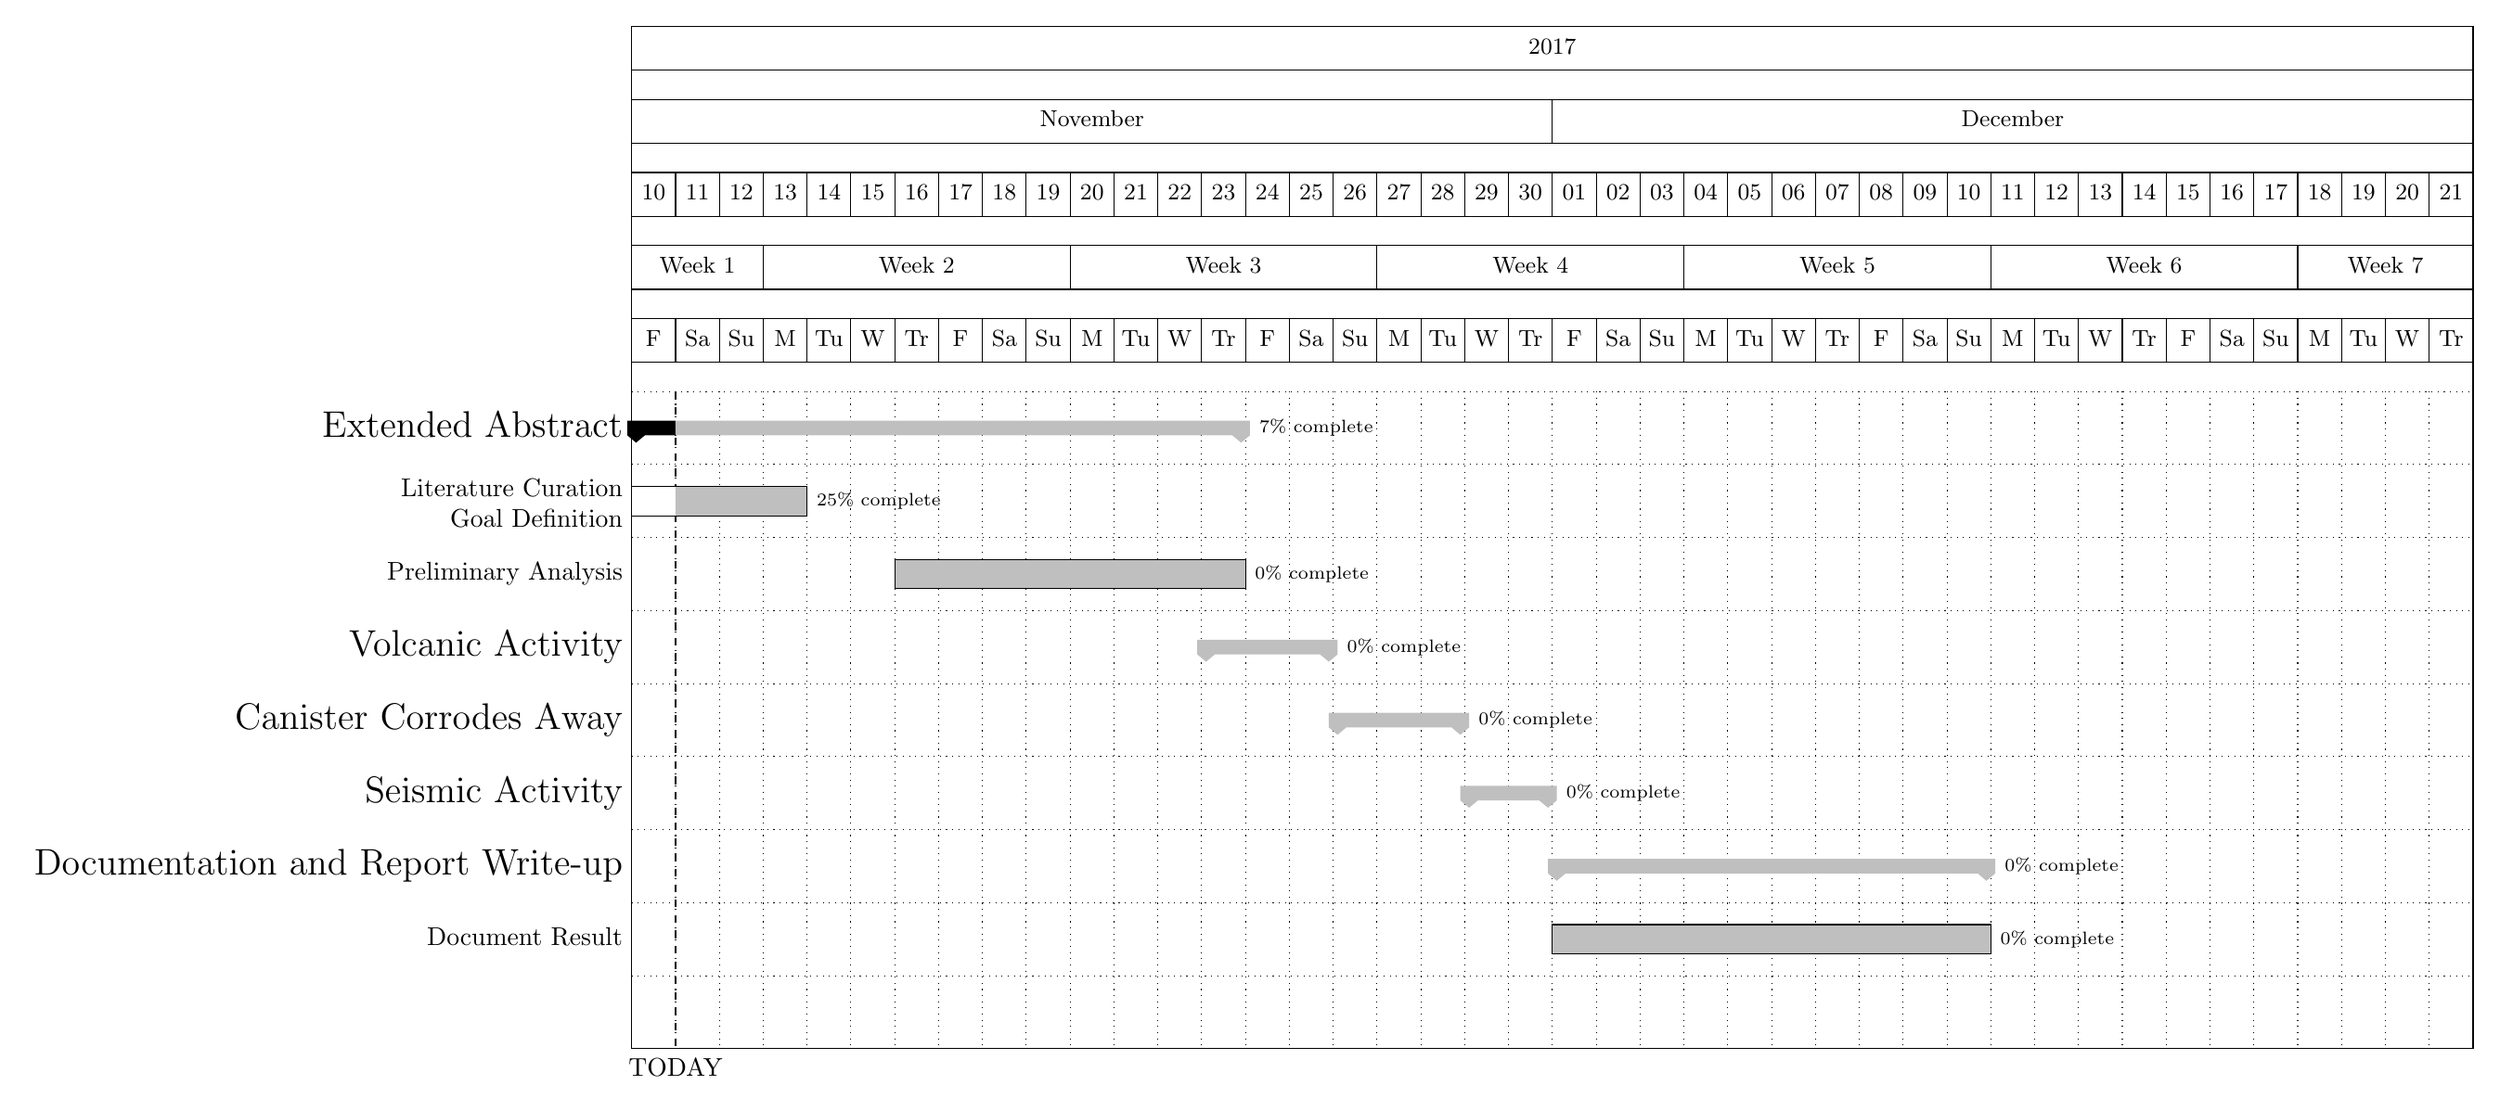
\begin{tikzpicture}[x=.5cm, y=1cm]
\begin{ganttchart}[
    hgrid,
    vgrid,
    group label font=\Large,
    progress=today,
    today=2017-11-10,
    x unit=6mm,
    newline shortcut=true,
    bar label node/.append style={align=right},
    time slot format=isodate
    ]{2017-11-10}{2017-12-21}
    \gantttitlecalendar{year, month=name, day, week=1, weekday=letter} \\
    
    \ganttgroup{Extended Abstract}{2017-11-10}{2017-11-23} \\
    \ganttbar{Literature Curation \ganttalignnewline Goal Definition}{2017-11-10}{2017-11-13} \\
    \ganttbar{Preliminary Analysis}{2017-11-16}{2017-11-23} \\

    
    \ganttgroup{Volcanic Activity}{2017-11-23}{2017-11-25} \\
    \ganttgroup{Canister Corrodes Away}{2017-11-26}{2017-11-28}\\
    \ganttgroup{Seismic Activity}{2017-11-29}{2017-11-30}\\
    \ganttgroup{Documentation and Report Write-up}{2017-12-01}{2017-12-10}\\
    \ganttbar{Document Result}{2017-12-01}{2017-12-10} \\
    
    

    
\end{ganttchart}
\end{tikzpicture}
}


\section{Background}
\gls{YMR} has been studied thoroughly in hopes of finally
disposing the U.S. \gls{UNF} inventory. However, considering
that it is a large project involving highly radioactive material,
careful planning and analyses must be done. The reference design
is taken from various sources \cite{u.s._department_of_energy_office_of_civilian_radioactive_waste_management_national_2008, wilson_total-system_1994, rechard_evolution_2014, u.s._department_of_energy_yucca_2002}.
Major sources of risk events are identified along with different ways to model
the events. 

Many risk events and components can be modeled using traditional methods like
failure probability from empirical tests and Human Reliability Analysis.
For simple mechanical procedures, for example, there exists previous data
on operation and failure probabilities. 

However, certain events are identified to be extremely difficult
to model using traditional risk analysis models. The events either
contain geological timescales or unpredictable natural disasters.
These events call for non-traditional methods of risk analysis.


\section{Literature Review}
System designs of the \gls{YMR} are listed extensively in literature \cite{u.s._department_of_energy_office_of_civilian_radioactive_waste_management_national_2008, wilson_total-system_1994, rechard_evolution_2014, u.s._department_of_energy_yucca_2002}, and contain multiple
iterations on the design. The basic design is as follows: the spent fuel assemblies
are repackaged in the waste package canister, and then placed underground,
underneath a drip shield. The canisters will remain there for up to millions of years,
surrounded by volcanic tuff.

Some prominent risk factors have also been identified. Volcanic hazards \cite{ho_risk_1992, smith_area_1990}
have been identified to be a long-term issue. Groundwater movement and transport of 
radioactive isotopes are another issue, in the case of canister breach \cite{robison_ground-water_1984, quade_fossil_1995}.  Canister reliability is another
identified risk factor \cite{whipple_can_1996, rutqvist_analysis_2003}.

Different aspects of risk analysis for nuclear waste repositories are published.
For systems where the future is hardly predictable, bayesian network analyses are 
suggested in \cite{lee_application_2006}. A method for sensitivity analysis
to rank important parameters are suggested in \cite{mohanty_cdf_2001}.


\section{Method}

For various facilities and aspects of the \gls{YMR}, imitating events that
cannot be modeled with traditional risk analysis methods are picked.
Those events are carefully analyzed and defined to find an adequate
method to model the events. Various literature will be curated for
reference. Then the analysis methods are carefully evaluated and reviewed.

\section{Definition of System Failure}
The definition of `System Failure' as a whole is tricky, but for this analysis it is defined
as `Radioactive Material Escape from Container.'
`Radioactive Material' would namely mean the spent fuel assemblies.
The container could be the transport cask which transports the assemblies from
the reactors to the site, or the emplacement cask, which is ultimately put in the repository.

\section{Definition of Initiating Event}
An initiating event is what causes a cascade of events that eventually leads
to the system failure, which is defined above as `Radioactive Material Escape
from Container'. Examples of initiating events are volcanic activity and 
earthquakes.

\section{System Analysis}
In order to identify the various initiating events, a thorough system analysis
is done. Among them, weaker points are emphasized to find the most severe
initiating event that will affect multiple facilities or components. 

Initiating events have been identified as crucial to the 
\gls{YMR} system are listed in table \ref{tab:ie}.

\begin{table}[h]
    \centering
%   \scalebox{0.86}{
        \begin{tabular}{ccc}
            \hline
            \textbf{Initiating Event} & \textbf{Reason} & \textbf{Difficulty to Model} \\ \hline
            Volcanic Activity & Repository rupture and Large Heat Influx & Rare event and needs modeling of physical phenomena \\ 
            Canister Corrodes Away & Leakage of Radioactive material & Modeling corrosion in geological time periods \\
            Seismic Activity & Repository rupture & Rare event and difficult to predict \\ \hline
        \end{tabular}
        \caption{List of initiating events crucial to the failure of the \gls{YMR}}
        \label{tab:ie}
\end {table}

The three initiating events all have very little data
and cannot have empirical data for modeling. Thus,
various methods have been used in an attempt to model these events.

\section{Goal}
The goal of this project is to research a method for effectively
modeling the three initiating events through literature review.
Preferably a value judgment will be made on the best method
for modeling the initiating event. 

\FloatBarrier



\section{Volcanic Activity}
Yucca Mountain has been considered a potential site
for volcanic activity due to its multiple basalt centers 
of Quaternary age \cite{management_environmental_1986}.
Many papers \cite{crowe_volcanism:_2006, crowe_status_1995}claim that
the presence of those volcanic rocks are a result of early volcanic episodes in the region,
and that a volcanic activity is likely to occur.
There also is not a recorded volcanism near Yucca Mountain, which required
detailed volcanologic studies to be done to obtain the history of 
volcanic activity in the region.

\subsection{Simple Poisson Method}
The first attempt to calculate the probability of volcanic disruption
at Yucca Mountain was Crowe and Carr \cite{crowe_preliminary_1980}, using 
a simple Poisson model:
\[P_r = exp(-\lambda t p)\]
\[\lambda = \text{recurrence rate of volcanic events}\]
\[p = \text{probability of a repository disruption, given a volcanic eruption}\]

This model assumed three things:

\begin{itemize}
    \item 1. Volcanic eruptions in successive time periods are independent
     and should follow Poisson distribution with constant mean\\
    \item 2. Every eruption has the same probability to disrupt the repository \\
    \item 3. Disruption events are independent \\
\end{itemize}

This model, using a refined mathematical model, resulted in a 
probability of volcanic disruption of the repository in the range of 
3.3e-10 to 4.7e-8 for the first year, with a linear increase with time \cite{crowe_volcanic_1986}.

Though a brave feat, the poisson model was not an adequate model for 
measuring a complex phenomenon like a volcanic eruption. The reasons
are the following:

\begin{itemize}
    \item 1. A simple Poisson model has a constant rate, which should be changing in time. Volcanic
            activities are considered "waning", "random", and "developing" in time \cite{ho_nonhomogeneous_1991}, meaning
            that the rate ($\lambda$) changes over time. 
    \item 2. Clear understanding is needed of eruptive processes and reliable dating techniques.
\end{itemize}


\subsection{Non-homogeneous Poisson Method}
An improvement from the simple Poisson model was made by using
non-homogeneous Poisson process with Weibull intensity \cite{ho_risk_1992}.
This process estimates the instantaneous recurrence rate using the
non-homogeneous Poisson process with Weibull intensity, and uses 
a homogeneous Poisson process to predict future eruptions.
Then, Bayesian analysis is performed to model the repository-disruptive frequency
given a volcanic eruption. This process replaces the constant $\lambda$ with
a time-dependent $\lambda(t)$. In the paper \cite{ho_risk_1992}, their choice of 
$\lambda(t)$ was the following:
\[ \lambda(t) = (\frac{t}{\theta})^{\beta}\]
which the first occurrenct follows a Weibull distribution, given by equation:
\[f(x;\lambda, k) = \frac{k}{\lambda} (\frac{x}{\lambda})^{k-1} for x\geq 0 \]

for different `stages', the $\beta$ holds different values, listed in table \ref{tab:beta}:

\begin{table}[h]
    \centering
%   \scalebox{0.86}{
        \begin{tabular}{cc}
            \hline
            \textbf{Volcano} & \textbf{$\beta$} \\ \hline
            Waning & 0.63 \\
            Random & 0.99 \\
            Developing & 5.40 \\
            \hline
       \end{tabular}
        \caption{Beta Values for different stages of volcanic period. If beta is larger than
                 1, the rate of eruption increases with time.}
        \label{tab:beta}
\end {table}

With the new $\lambda$ estimated, that $\lambda$ is plugged into simple Poisson distribution
(homogeneous Poisson) to calculate recurrence rate ($\lambda(t) t_0 $) for future time $[t, t+t_0]$.
This non-homogeneous Poisson method with updated eruption rate is to take into account both the 
specific physical events or processes that cause volcanic eruptions ($\lambda(t)$), and the 
various factors with random influences (Simple Poisson).

\begin{wrapfigure}{r}{0.4\textwidth}
\centering
\caption{This map outlines the are of most recent volcanic activity (dashed line)
and high-risk zones (rectangles). The dark shape labeled YM is the repository.}

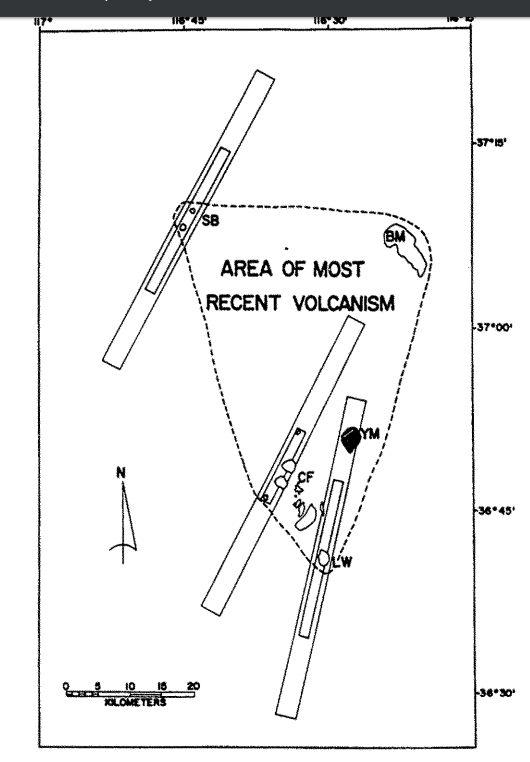
\includegraphics[scale=0.3]{./images/map.png}
\vspace{-10pt}
\label{fig:map}

\end{wrapfigure}


For the probability of the volcanic eruption disrupting the repository, a map is drawn
with the area of most recent volcanic activity to identify high-risk zones (Figure \ref{fig:map}).
The proportion of the repository that is inside the risk zone is then used
for the upper limit for the probability.


The non-homogeneous Poisson method included various physical events and historic eruptions
into its risk calculation, as well as reflect the randomness of volcanic eruptions.
This resulted in a 90\% confidence interval for the probability of `site disruption'
of 0.01 to 0.067 for 10,000 years \cite{ho_risk_1992}.

\subsection{Multiple non-homogeneous Poisson models}
Connor et al. proposed a three non-homogeneous Poisson model
to model volcanic activity in Yucca Mountain \cite{connor_three_1995}.
The three methods are: spatio-temporal nearest neighbor,
kernel and nearest-neighbor kernel. The combination provides
the following benefits:
\begin{itemize}
    \item Recurrence rate and probability can be mapped \\
    \item No need to define areas of zones of volcanic activity \\
    \item Impact of uncertainty in timing and distribution is easy \\
\end{itemize}

This model incorporates more physical events and geological data 
in order to construct the three methods. The details of constructing 
the estimates with geological data (rock age, maps) is beyond the scope
of this review.

In short, this more detailed model takes into account the 
clustering of Quaternary volcanoes and the spatial dependency
or volcanic recurrence. This model resulted in a probability
of disruption within the 8 square kilometers of the repository
between 0.0001 and 0.0005 in 10,000 years \cite{connor_three_1995}.


\subsection{Discussion}
The evolution of the methods of predicting volcanic eruption
and its probability to disrupt the repository was mainly
the evolution of taking into account various physical phenomenon
that change over time. Given geological timescales and lack
of historical data, predictions could only be made from current
geological formations that hint at a possibility of volcanic formation.
The reviewed papers progressively added layers and layers of geologic
and physical contribution to volcanic eruption, to add complexity to
their models.

Given a detailed geological database of the region and a clear understanding
of volcanic formation and activity, a Monte Carlo method can be an 
improvement from these multiple Poisson methods, where the entire
region can be simulated and tested to see if the repository is disrupted
in 10,000 years. However, such as feat would cost tremendous resources,
which would call for estimates and assumptions.  


\FloatBarrier


\pagebreak



\bibliographystyle{unsrtnat}
\bibliography{bibliography}


\end{document}
\grid
